\documentclass[a4paper,12pt]{report}

\usepackage{alltt, fancyvrb, url}
\usepackage{graphicx}
\usepackage[utf8]{inputenc}
\usepackage{float}
\usepackage{hyperref}

% Questo commentalo se vuoi scrivere in inglese.
\usepackage[italian]{babel}

\usepackage[italian]{cleveref}

\title{Relazione\\''Unibo-td''}

\author{Aurora Francesco \\ 
Casali Marco \\
Murvai Cristina \\
Pulga Luca}
\date{07 luglio 2024}


\begin{document}

\maketitle

\tableofcontents

\chapter{Analisi}
"Bloons Tower Defense" è una serie di videogiochi di tipo tower defense. In questi giochi, il giocatore deve posizionare diverse torri lungo un percorso per fermare ondate di palloncini (chiamati "bloons") che cercano di attraversarlo. Ogni "bloon" che raggiunge la fine del percorso fa perdere una vita al giocatore, e il gioco termina quando le vite scendono a zero.
\\
\\
Il software mira ad una imitazione di questo videogioco. La nostra implementazione presenta alcune limitazioni e semplificazioni rispetto alla complessità del gioco originale. Questo ci ha permesso di comprendere meglio le dinamiche e le sfide dello sviluppo di un videogioco tower defense, anche se con risultati meno sofisticati rispetto alla versione commerciale.

\section{Requisiti}

Il gioco è implementato a round di difficoltà incrementale in cui i giocatori cercano di impedire ai nemici di raggiungere la fine di un percorso stabilito, posizionando difese per eliminarli. \\
Eliminando i nemici si guadagnano monete che possono essere utilizzate per acquistare nuove difese.\\
Si hanno a disposizione N vite, che si decrementano quando i nemici raggiungono la fine del percorso.\\
Quando si arriva a 0 vite il gioco termina.

\subsection*{Requisiti funzionali}
\begin{itemize}
	\item Il gioco inizia mostrando la schermata di avvio, in seguito è possibile scegliere la tipologia di mappa per iniziare la partita.
	\item Scelta la mappa, viene mostrata l’area di gioco: questa consiste in una griglia in cui il giocatore può posizionare le proprie difese (torri) in un determinato tempo prima che inizi ad arrivare la prima ondata di nemici. A sinistra della griglia si trovano le torri posizionabili nella mappa, in alto, invece, vengono indicate le vite, il round, il timer e i soldi guadagnati.
	\item Il gioco è suddiviso in round con difficoltà incrementale.
	\item I nemici sono le entità che seguono il percorso sulla mappa alla stessa velocità con lo scopo di giungere al termine, senza essere uccisi dalle difese.
	\item Il giocatore può piazzare torri lungo il percorso nei punti permessi per difendersi dai nemici.
	\item Ogni difesa ha a disposizione una e una sola arma.
	\item Le torri colpiscono i nemici quando entrano nel loro raggio di azione.
	\item I nemici hanno un life point che viene decrementato ogni volta che una torre riesce a colpire il nemico. Quando il life point diventa zero, il nemico risulta sconfitto e si vince una ricompensa (denaro) che può essere utilizzata per acquistare altre difese.
	\item Viene quindi gestito un sistema di reward dei nemici sconfitti e perdita delle vite del giocatore.
\end{itemize}

\subsection*{Requisiti non funzionali}
\begin{itemize}
	\item Garantire fluidità del gioco su diverse piattaforme.
	\item Assicurare che il gioco sia compatibile con le versioni dei principali sistemi operativi (Windows, Linux, macOS).
\end{itemize}
\newpage
\section{Analisi e modello del dominio}



\chapter{Design}

\section{Architettura}

UNIBO-TD adotta il pattern architetturale MVC. Il Model, una volta avviato dal Controller, esternalizza e gestisce in modo trasparente la logica tramite il defense manager e l'enemy manager, i quali si occupano di aspetti diversi del gioco, come i nemici e le difese. Il Controller funge da intermediario tra Model e View, limitando l'accesso diretto al Model e fornendo solo oggetti di trasferimento dati. Ciò significa che gli altri componenti dell'applicazione, come la View, possono accedere solo a una rappresentazione immutabile dei dati nel Model, garantendo un maggiore controllo sull'integrità dei dati. Di conseguenza, l'implementazione della View, così come è stata definita, è facilmente sostituibile poiché non dipende dalle classi sottostanti.





\section{Design dettagliato}
\subsection{Francesco Aurora}
\title{\textbf{Gestione GUI e azioni utente, round, player}}
\subsubsection{Gestione Round}
\begin{figure}[H]
	\centering{}
	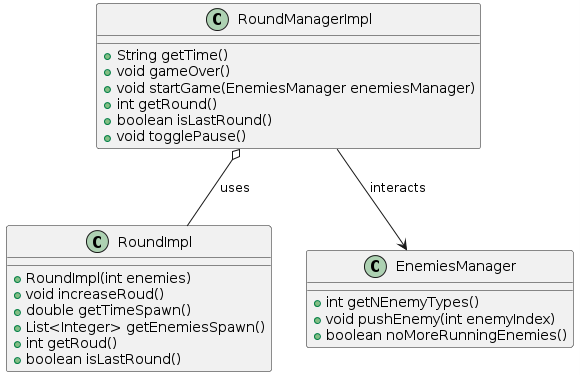
\includegraphics{docs\RelazioneTD\images\Round.png}
	\caption{UML relazioni Round}
	\label{img:Gui}
\end{figure}
\paragraph{Problema} Nel contesto di un gioco a round, è essenziale gestire in modo efficace la progressione dei round e la generazione dei nemici. Il problema principale consiste nel determinare come incrementare il numero di round, regolare il numero di nemici generati, gestire i tempi di spawn dei nemici e differenziare i round normali dai "boss round". Inoltre, la gestione del gioco deve includere la capacità di mettere in pausa, riprendere e interrompere il gioco in modo sicuro, sincronizzando correttamente l'accesso ai dati condivisi tra i thread per evitare condizioni di gara e inconsistenze.

\paragraph{Soluzione} Per affrontare questi problemi, ho progettato un sistema che utilizza due classi principali: \texttt{RoundImpl} e \texttt{RoundManagerImpl}.

\texttt{RoundImpl} gestisce la logica interna dei round, inizializzando il numero di nemici, il tempo di spawn e una lista di nemici. Il metodo \texttt{increaseRoud()} gestisce l'incremento dei round, aggiornando la lista dei nemici e modificando il tempo di spawn a seconda del tipo di round.

\texttt{RoundManagerImpl} gestisce il flusso del gioco, inclusi il countdown e la generazione sequenziale dei nemici, utilizzando due thread distinti. Il metodo \texttt{togglePause()} gestisce la pausa e la ripresa del gioco in modo sicuro. La sincronizzazione dei dati tra i thread è garantita da blocchi di sincronizzazione.

Ho valutato l'alternativa di gestire tutti i round e i nemici in una sola classe, ma ho optato per la separazione per migliorare la modularità e la chiarezza del codice. Utilizzare thread distinti per il countdown e la generazione dei nemici ha migliorato la gestione del flusso di gioco e facilitato la manutenzione ed estensione del sistema.

Questo design offre un sistema robusto e flessibile, risolvendo efficacemente i problemi identificati e migliorando l'esperienza di gioco complessiva.

\subsubsection{Gestione player}
\begin{figure}[H]
	\centering{}
	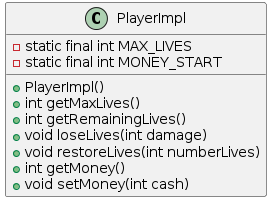
\includegraphics{docs\RelazioneTD\images\Player.png}
	\caption{UML player}
	\label{img:Gui}
\end{figure}
\paragraph{Problema} Nel contesto di un gioco, è essenziale gestire lo stato del giocatore, compreso il numero di vite rimanenti e il denaro disponibile. Il problema principale consiste nel mantenere aggiornati questi due attributi in base alle azioni del giocatore e agli eventi nel gioco.
\paragraph{Soluzione} Per affrontare questo requisito, ho progettato la classe PlayerImpl. Questa classe implementa l'interfaccia Player, fornendo metodi essenziali per gestire le vite e il denaro del giocatore. Il costruttore inizializza il giocatore con un numero massimo di vite e un quantitativo iniziale di denaro. I metodi loseLives(int damage) e restoreLives(int numberLives) aggiornano le vite del giocatore in base ai danni subiti o al ripristino delle vite. Allo stesso modo, i metodi getMoney() e setMoney(int cash) gestiscono il denaro del giocatore, consentendo di recuperare la quantità di denaro attuale e aggiornarla in base alle transazioni nel gioco.

Questa progettazione garantisce un controllo efficace e dinamico sulle risorse del giocatore, fondamentale per una esperienza di gioco coinvolgente e bilanciata.

\subsubsection{Gestione della Schermata di Avvio e Selezione Mappa}
\begin{figure}[H]
	\centering{}
	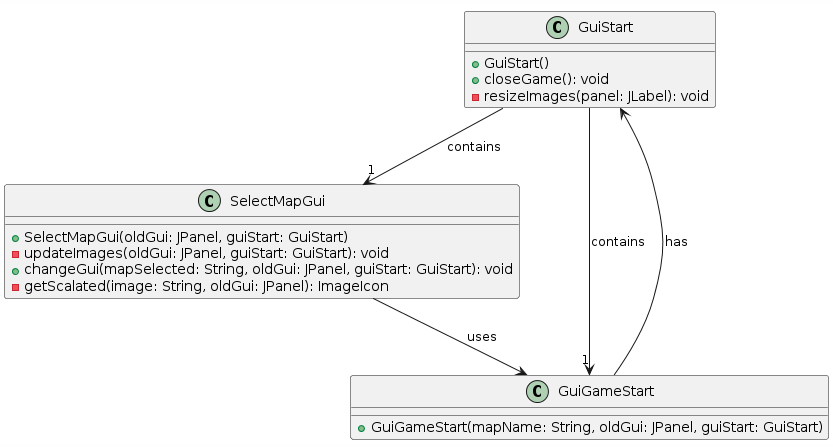
\includegraphics{docs\RelazioneTD\images\Gui.png}
	\caption{UML relazioni GUI}
	\label{img:Gui}
\end{figure}
\paragraph{Problema} Nell'implementazione di un'applicazione GUI per un gioco, è essenziale gestire efficacemente la schermata iniziale, includendo un pulsante di avvio ben posizionato e scalabile per adattarsi a diverse dimensioni di scherma, la selezione delle mappe ancora adattabile a diverse dimensioni dello schermo. Il problema principale consiste nel progettare un'interfaccia utente che permetta agli utenti di selezionare una mappa tra diverse opzioni, visualizzare anteprime delle mappe adattate alle dimensioni dello schermo e fornire un'esperienza utente coerente e intuitiva su diversi dispositivi.
\paragraph{Soluzione} Le classi `GuiStart` e `SelectMapGui` sono componenti chiave nell'interfaccia utente del gioco. `GuiStart` gestisce la schermata iniziale, impostando il titolo della finestra su "Unibo TD", utilizzando `BorderLayout` per organizzare i componenti e includendo un pulsante di avvio. `SelectMapGui` gestisce la selezione della mappa, permettendo agli utenti di scorrere tra le mappe disponibili e avviare il gioco con la mappa selezionata.

Entrambe le classi sono progettate per essere responsive, adattandosi automaticamente alle dimensioni dello schermo per garantire una esperienza utente ottimale.

Questa soluzione offre un'interfaccia utente ben strutturata e facile da navigare, ottimizzata per migliorare l'esperienza dell'utente fin dai primi istanti di utilizzo del gioco. È progettata per consentire una transizione fluida tra diverse schermate, inclusa quella del gioco vero e proprio, all'interno della stessa finestra.

Come futura implementazione, si potrebbe considerare l'integrazione degli effetti sonori e la visualizzazione di più mappe simultaneamente sullo schermo, al fine di offrire agli utenti una visione più completa e coinvolgente delle opzioni di gioco disponibili.

\subsubsection{Schermata di gioco Mappa}
\begin{figure}[H]
	\centering{}
	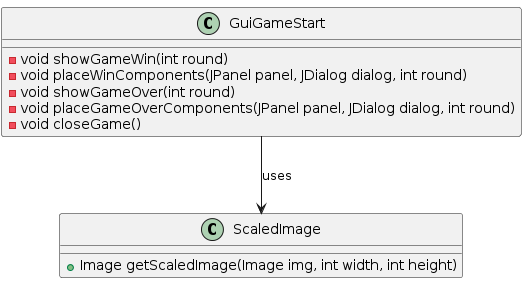
\includegraphics{docs\RelazioneTD\images\GuiGameStart.png}
	\caption{UML GUI mappa per area di mia pertinenza}
	\label{img:GuiGameStart-Aurora}
\end{figure}
\paragraph{Problema} Si vuole gestione la vittoria e sconfitta, resize della mappa all'adattamento della finestra, bottoni pausa e settings.
\paragraph{Soluzione} La mappa viene ridimensionata tramite l'evento di \texttt{resize} ogni volta che il contenitore delle immagini della mappa cambia dimensione. La gestione della vittoria e della sconfitta è implementata in modo tale che, quando il core rileva eventi di \texttt{GameOver} o \texttt{GameWin}, viene mostrato un \texttt{JDialog}. Al clic sul pulsante \texttt{exit}, viene generato l'evento di chiusura del gioco. Poiché le pagine sono state incapsulate, l'evento deve essere richiamato sulla prima GUI mostrata. Il tutto deve essere scalabile tramite l'utilizzo di metodi in cascata e non ridondante. La suddivisione dei due metodi per \texttt{gameWin} e \texttt{gameOver} permette, in futuro, di avviare comportamenti diversi e di gestire in modo appropriato eventuali store di dati.

Nella schermata di gioco sono stati aggiunti i pulsanti \texttt{pausa} e \texttt{impostazioni}. Il pulsante \texttt{pausa} avvia una chiamata al core di gioco per mettere in pausa i vari componenti del gioco. Il pulsante \texttt{impostazioni} attualmente non è funzionante, poiché non sono stati ancora gestiti gli effetti sonori e la velocità di gioco. In futuro, si potrebbe implementare il pulsante \texttt{impostazioni} per mettere in pausa il gioco e permettere di configurare questi aspetti.
\newpage
\subsection{Marco Casali}
\title{\textbf{Game loop, generazione mappa}}




\newpage
\subsection{Cristina Murvai}
\subsubsection{Gestione delle diverse configurazioni di nemici}
\begin{figure}[H]
    \centering
    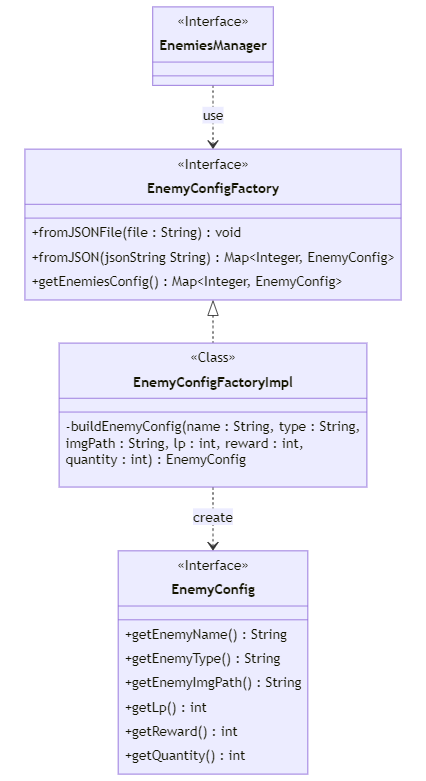
\includegraphics[scale=0.8]{RelazioneTD/images/enemyConfigFactoryUML.png}
    \caption{UML factory per caricamento di configurazioni di nemici}
    \label{fig:enter-label}
\end{figure}

\paragraph{Problema} Il gioco prevede attualmente tre tipologie di nemici, ciascuno con paramentri diversi quali il nome, i punti vita, il reward assegnato con l'uccisione, ecc. che è necessario reperire ogni volta in cui un nemico di quella tipologia viene creato. 
\paragraph{Soluzione} Per garantire futura estendibilità ad ulteriori tipologie di nemici e facile modifica dei parametri è stato deciso di gestire la configurazione dei nemici attraverso un file JSON. Tuttavia, una lettura di questo file in seguito alla creazione di ciascun nemico sarebbe inutilmente dispendiosa del punto di vista delle risorse del sistema. Per questo motivo, si è deciso di sfruttare il pattern factory per creare e salvare in memoria i dati relativi alle varie tipologie di nemici, garantendo un accesso più rapido in fase di generazione degli stessi tramite il metodo \textit{getEnemiesConfig()} dell'interfaccia \textit{EnemyConfigFactory}. In particolare il metodo \textit{fromJSONFile()} è sfruttato da \textit{EnemiesManager} per leggere il file di configurazione e creare attraverso la factory i diversi \textit{EnemyConfig}.

\subsubsection{Gestione dei nemici: spawn, movimento e distruzione}

\begin{figure}[H]
    \centering
    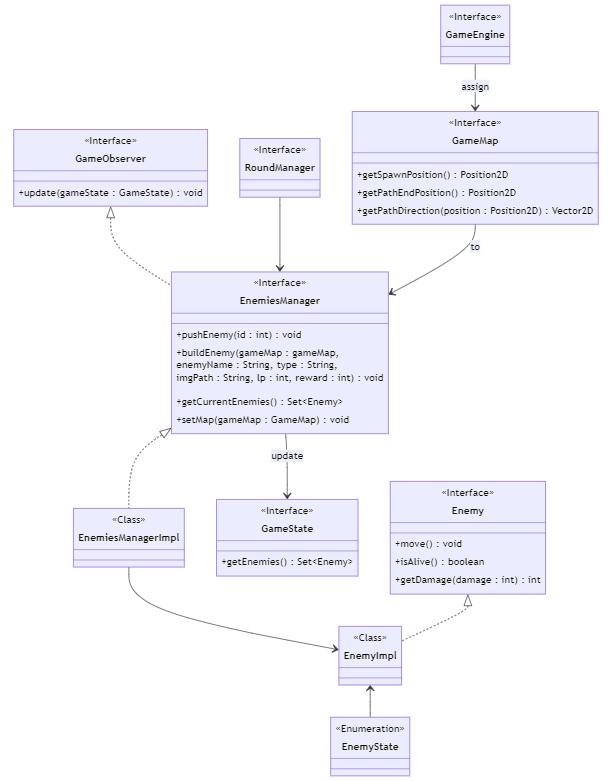
\includegraphics[scale=0.8]{RelazioneTD/images/enemiesManagerUML.png}
    \caption{UML gestione dei nemici}
    \label{fig:enter-label}
\end{figure}

\paragraph{Problema} Per poter correttamente gestire la creazione e il movimento dei nemici è necessario avere informazioni riguardo la mappa quali posizione di partenza, percorso da seguire e fine del percorso.

\paragraph{Soluzione} Dato che la scelta della mappa viene fatta in un secondo momento rispetto all'avvio del gioco, si è deciso di avviare comunque l'\textit{EnemiesManager} in modo tale da eseguire immediatamente il load delle diverse configurazioni di nemici descritto al punto precedente. Per questo motivo si è scelto di modellare \textit{GameMap} per il manager dei nemici con tipo \textit{Optional}, il cui valore viene assegnato dal \textit{GameEngine} appena l'utente effettua la selezione della mappa di gioco avviando la partita.

\paragraph{Problema} Per la gestione delle interazioni difese-nemici si è reso necessario fornire al manager delle difese un modo efficace per monitorare quali nemici sono in vita e conoscere la loro posizione in tempo reale. Questo è cruciale per permettere alle torri di attaccare correttamente i nemici.

\paragraph{Soluzione} Si è deciso di sfruttare il pattern Observer per risolvere questo problema, rendendo il set dei nemici osservabile. Questo set è disponibile nell'interfaccia \textit{GameState} e qualsiasi componente che necessita di monitorare i nemici, come il manager delle difese, può iscriversi come osservatore. Ogni volta che c'è un cambiamento nel set dei nemici (ad esempio, un nemico viene eliminato o cambia posizione), gli osservatori vengono notificati e possono conseguentemente aggiornare il loro stato. Ciò garantisce che tutte le parti del sistema che devono reagire ai cambiamenti dello stato dei nemici lo facciano immediatamente e in modo coerente. Inoltre, questo rende il codice scalabile, poiché è possibile aggiungere nuovi osservatori dello stato dei nemici senza modificare il codice sorgente esistente.

\paragraph{Problema} Il \textit{RoundManager} si occupa della gestione dei vari round e quindi anche di stabilire il numero incrementale di nemici di diverse tipologie che popoleranno la mappa di gioco. Per questo motivo è necessario fornirgli un modo per generare i nemici in maniera efficace. Per fare ciò è necessario anche considerare che, visto che \textit{EnemiesManager} estende \textit{GameObserver}, il set dei nemici potrà essere modificato solo quando il manager avrà il controllo nel metodo \textit{update()}.

\paragraph{Soluzione} Per risolvere questo problema si è deciso di fornire al \textit{RoundManager}, tramite \textit{EnemiesManager}, il metodo \textit{pushEnemy()} che, preso in ingresso l'identificativo di una tipologia di nemici, tramite \textit{buildEnemy()} si occupa di creare un nuovo nemico. L'\textit{EnemiesManager} inizializza poi la posizione del nemico, utilizzando i metodi forniti da \textit{GameMap}, e lo aggiunge ad un set temporaneo di nemici da inserire nella partita. Una volta che il manager ha il controllo sul set dei nemici, ovvero quando il \textit{GameEngine} ne chiama il metodo \textit{update()}, i nemici presenti nel set temporaneo vengono aggiunti a quello effettivo e il loro movimento sulla mappa inizia rendendoli anche colpibili dalle difese.

\subsubsection{Gestione visualizzazione grafica dei nemici}
\paragraph{TO-DO}


\newpage
\subsection{Luca Pulga}
\subsubsection{Gestione delle difese}
\paragraph{Problema}
Si vuole gestire in maniera scalabile le varie entità presenti all'interno del gioco, come le difese (torri, armi, proiettili) e i nemici, evitando l'eccessiva scrittura di codice duplicato.

\paragraph{Soluzione}
E' possibile suddividere le varie caratteristiche delle varie entità in sotto-entità, in modo da attribuire le relative proprietà ad ogni tipologia di entità che è presente
o che potrà essere presente in futuro, rendendo la struttura scalabile. Sono state realizzate interfacce e classi astratte, a cui sono state delegate le assegnazioni delle varie proprietà, fornendo la condivisione del codice comune e contratti parziali, implementabili dalle sottoclassi.
Un'ulteriore soluzione poteva essere quella di utilizzare solo interfacce e come implementazione di esse utilizzare i record, in quanto fornirebbero un modo decisamente più coinciso per dichiarare classi immutabili ed eliminerebbero molta della verbosità associata alle classi standard.

\begin{figure}[H]
    \centering
    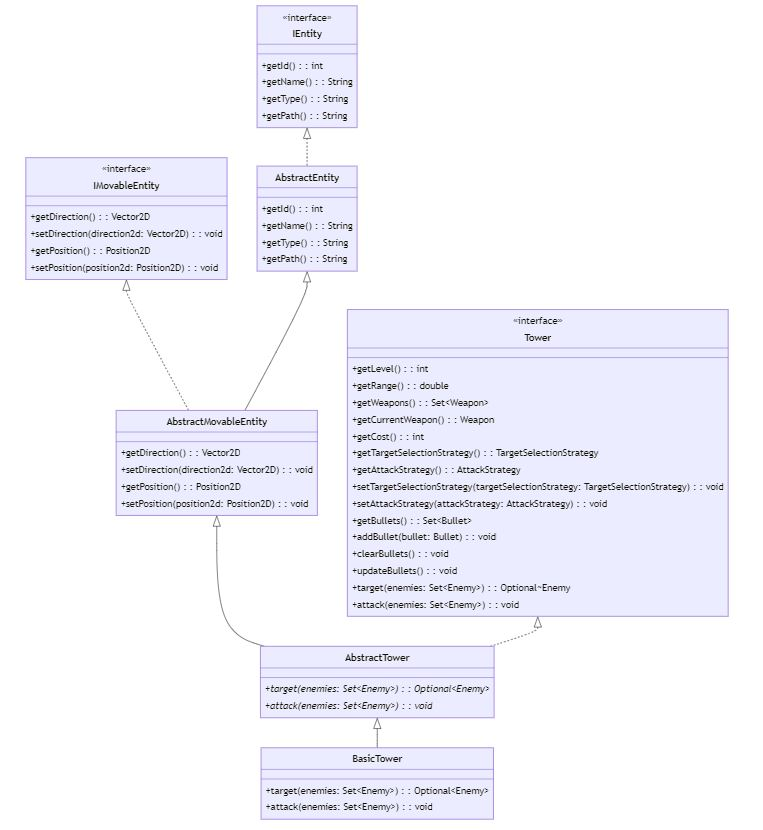
\includegraphics[width=1.2\linewidth]{defense_model.JPG}
    \caption{Modello per la gestione delle entità.}
    \label{fig:defense-model}
\end{figure}

\vspace{15mm}

\paragraph{Problema}
Disporre di un oggetto in grado di poter creare qualsiasi tipo di entità, centralizzando la parte di creazione degli oggetti che verranno caricati e successivamente utilizzati durante il gioco.

\paragraph{Soluzione}
Si utilizza il \textit{Factory Method Pattern} in modo da sfruttare la sua capacità di separare la costruzione degli oggetti dal loro utilizzo. Dunque questa separazione ci consente di avere una maggiore flessibilità e modularità del codice, rendendolo più facile da mantenere e aggiornare anche introducendo in futuro nuove entità o separare in sotto-entità quelle già esistenti. 
La \textit{Factory} provvederà a leggere i files json all'interno di specifiche cartelle per caricare
le entità, come le \textit{torri}, che saranno poi successivamente gestite dal \textit{Defense Manager}.


\begin{figure}[H]
    \centering
    
\includegraphics[width=0.8\linewidth]{todo.jpg}
    \caption{Factory Method Pattern per il caricamento delle entità.}
    \label{fig:entity-factory-method}
\end{figure}
\vspace{25mm}

\paragraph{Problema}
Gestione delle istanze delle torri senza avere un'entità centralizzata.
\paragraph{Soluzione}
La soluzione prevedere l'implementazione di un Defense Manager in grado di gestire le entità difesa. Questa soluzione centralizzata permette di gestire all'interno di un unica classe tutte le entità difesa, fornendo anche un modo comodo all'esterno per ottenere informazioni con altri oggetti.

\begin{figure}[H]
    \centering
    
\includegraphics[width=0.8\linewidth]{todo.jpg}
    \caption{Defense Manager per la gestione delle difese.}
    \label{fig:defense-manager}
\end{figure}

\vspace{50mm}
\paragraph{Problema}
Gestione di varie tipologie di entità in tempo reale come torri, proiettili, nemici e tutte le varie entità che potrebbero essere introdotte in futuro che hanno necessità di reagire a certi eventi.
\paragraph{Soluzione}
A livello di difese, si sottoscrive il Defense Manager all'Observer, il quale consente di definire un meccanismo di sottoscrizione per notificare a più oggetti gli eventi che accadono all'oggetto che stanno osservando, tutto ciò rispettando il principio Open/Closed, migliorando così la modularità e la manutenibilità del codice.

\begin{figure}[H]
    \centering
    
\includegraphics[width=0.8\linewidth]{todo.jpg}
    \caption{Figura 2.5: Defense Manager e Observer.}
    \label{fig:defense-observer}
\end{figure}
\vspace{50mm}


\paragraph{Problema}
Implementazione di diverse tipologie di targettamento dei nemici da parte delle torri a seconda della loro tipologia.
\paragraph{Soluzione}
Si implementa lo Strategy Pattern, in questo modo il contesto diventa indipendente dalle strategie concrete di targettamento dei nemici, per cui è possibile aggiungere/modificare gli algoritmi di targettamento senza modificare il codice all'interno delle varie classi che potrebbero implementare la relativa strategia di attacco.

\begin{figure}[H]
    \centering
    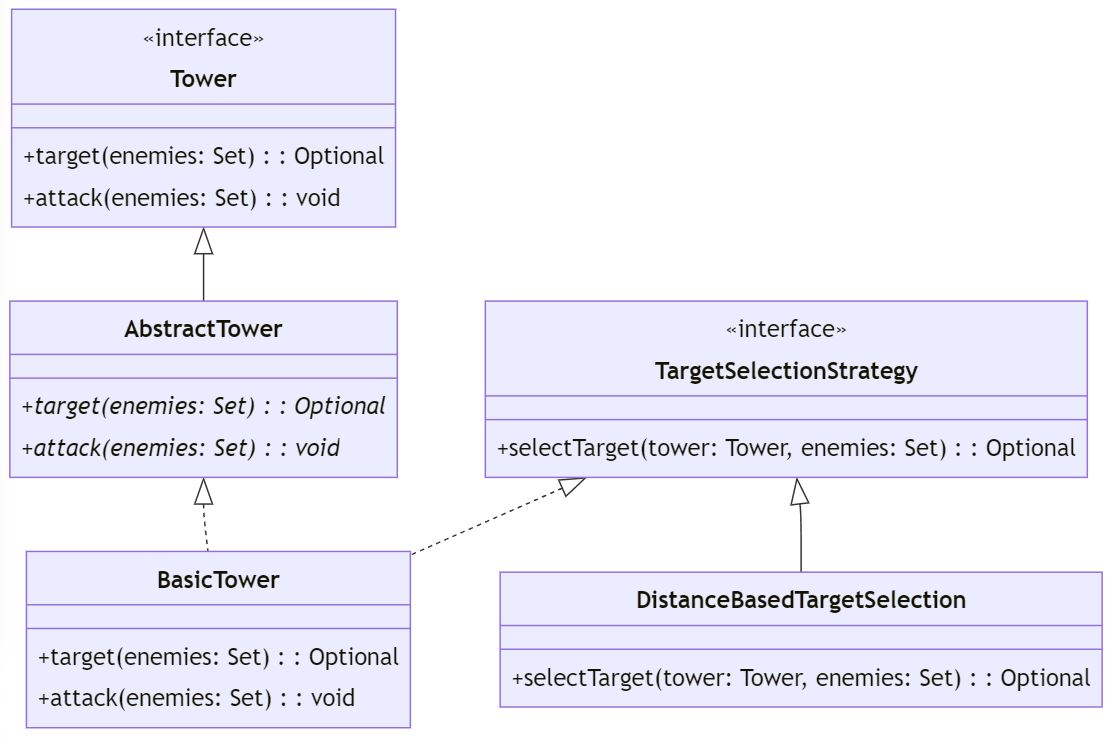
\includegraphics[width=0.8\linewidth]{defense_target.JPG}
    \caption{Pattern Strategy per targettamento dei nemici.}
    \label{fig:defense_target}
\end{figure}


\paragraph{Problema}
Implementazione di diverse tipologie di attacchi verso i nemici da parte delle torri a seconda della loro tipologia.
\paragraph{Soluzione}
Si implementa lo Strategy Pattern, in questo modo il contesto diventa indipendente dalle strategie concrete di attacco verso i nemici, per cui è possibile aggiungere/modificare gli algoritmi di attacco senza modificare il codice all'interno delle varie classi che potrebbero implementare la relativa strategia di attacco.

\begin{figure}[H]
    \centering
    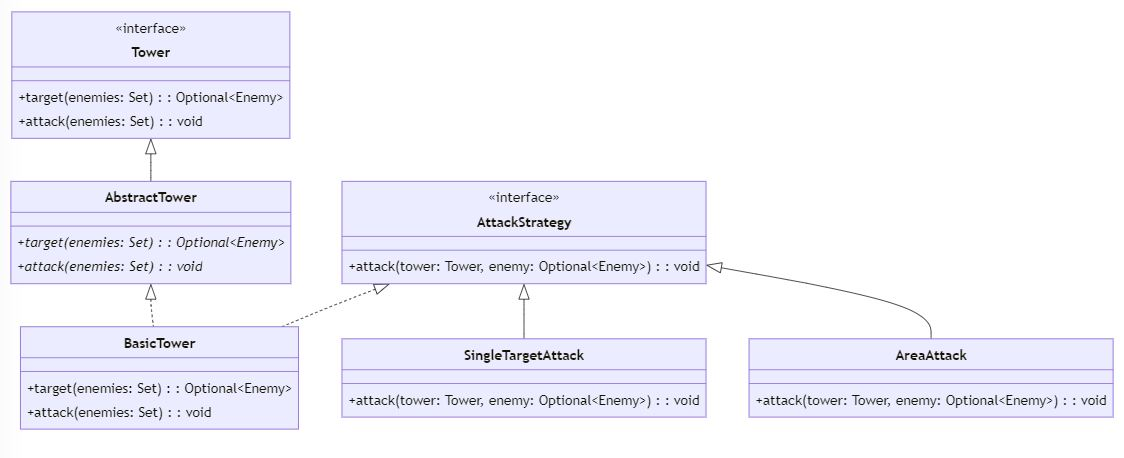
\includegraphics[width=0.8\linewidth]{defense_attack.JPG}
    \caption{Pattern Strategy per attacco ai nemici.}
    \label{fig:defense_attack}
\end{figure}

\chapter{Sviluppo}
\section{Testing automatizzato}
Per verificare il corretto funzionamento del gioco Tower-Defense, sono stati creati appositi test automatizzati utilizzando JUnit. 
I test automatizzati sono necessari per poter testare se le logiche pensate durante la fase analisi, di progettazione e di implementazione del Model, e delle classi affini di utility, sono funzionanti.


\begin{itemize}
    \item \textit{\textbf{TestBasicTower}:} Test automatizzato per garantire la correttezza dei metodi di get e set delle difese torri per poter gestire durante il gioco le sue proprietà.
    \item \textit{\textbf{TestBulletImpl}:} Test automatizzato per garantire la correttezza dei metodi di get e set della posizione e direzione del proiettile, fondamentale per la gestione grafica del gioco.
    \item \textit{\textbf{TestDefenseFactory}:} Test automatizzato per garantire la correttezza di lettura da file JSON delle entità torri attraverso l'utilizzo della \ref{fig:entity-factory-method}EntityFactory
    \item \textit{\textbf{TestTargetStrategy}:} Test automatizzato per garantire la correttezza dei calcoli effettuati durante la fase di targettamento di nemici da parte delle torri.
    \item \textit{\textbf{TestEnemiesConfigFactoryImpl}:} Test automatizzato per verificare la corretta funzionalità di caricamento delle configurazioni dei nemici da file JSON.
    \item \textit{\textbf{TestEnemyImpl}:} Test automatizzato per garantire il funzionamento di vari metodi della classe Enemy, come ad esempio verificare se lo stato iniziale, i punti vita, la ricompensa e il percorso dell'immagine sono impostati correttamente, oppure controllare se il nemico si muove lungo la direzione giusta,  aggiornando il suo stato una volta raggiunta la fine del percorso. 
	\item \textit{\textbf{TestPlayer}:} Test automatizzati per verificare la corretta inizializzazione di soldi e vite, nonché il corretto decremento e incremento di questi valori.
	\item \textit{\textbf{TestRound}:} Test automatici per verificare l'incremento dei round e della complessità del gioco.
	\item \textit{\textbf{TestRoundManagerImpl}:} Test automatici per verificare l'avvio del conto alla rovescia e l'avvio, oltre alla pausa del gioco.
\end{itemize}

\section{Note di sviluppo}

\subsection{Francesco Aurora}

\subsection{Marco Casali}
\subsection{Cristina Murvai}
\subsection{Luca Pulga}
\subsubsection{Utilizzo di Optional}
Utilizzati in vari punti. Un esempio: 
\url{https://github.com/PulgaLuca/OOP23-unibo-td/blob/12d7eec3c7e4b474e6f315461642e1c6a2d6c693/src/main/java/it/unibo/model/entities/defense/tower/target/DistanceBasedTargetSelection.java#L24}

\subsubsection{Utilizzo di generici}
\url{https://github.com/PulgaLuca/OOP23-unibo-td/blob/12d7eec3c7e4b474e6f315461642e1c6a2d6c693/src/main/java/it/unibo/model/entities/EntityFactoryImpl.java#L40}

\subsubsection{Utilizzo di lambda expressions}
Utilizzate in vari punti. Un esempio:  
\url{https://github.com/PulgaLuca/OOP23-unibo-td/blame/12d7eec3c7e4b474e6f315461642e1c6a2d6c693/src/main/java/it/unibo/model/entities/defense/manager/DefenseManagerImpl.java#L96}

\subsubsection{Utilizzo della libreria SLF4J}
Utilizzata in vari punti. Un esempio:  
\url{https://github.com/PulgaLuca/OOP23-unibo-td/blame/12d7eec3c7e4b474e6f315461642e1c6a2d6c693/src/main/java/it/unibo/model/entities/defense/manager/DefenseManagerImpl.java#L29C43-L29C43}

\subsubsection{Utilizzo della libreria Jackson per interazione con file JSON}
Un esempio:  
\url{https://github.com/PulgaLuca/OOP23-unibo-td/blob/12d7eec3c7e4b474e6f315461642e1c6a2d6c693/src/main/java/it/unibo/model/entities/EntityFactoryImpl.java#L66}



\chapter{Commenti finali}
\section{Autovalutazione e lavori futuri}
\subsubsection{Francesco Aurora}
\subsubsection{Marco Casali}
\subsubsection{Cristina Murvai}
\subsubsection{Luca Pulga}
\paragraph{}Prendere parte a questo progetto è stata un'attività non semplicissima ma decisamente formativa, soprattutto in ottica futura.
La progettazione della parte difensiva del gioco ricopre un ruolo massivo dell'applicazione e ho cercato non solo di cimentarmi nella mia parte di difese, ma anche nel cercare una generalizzazione relativamente alle varie tipologie di entità presenti nel gioco. La soluzione adottata rende estendibile il codice in caso di futuri sviluppi, attraverso l'astrazione delle entità e all'utilizzo di Design Patterns fondamentali per rendere il codice maggiormente leggibile e scalabile. Purtroppo non sono riuscito a sfruttare a pieno la programmazione funzionale e altre tecniche di programmazione illustrate durante il corso, che mi sarebbe interessato implementare e progettare, ma che porto ora con me nel mio bagaglio formativo. Non sono totalmente appagato dalla UX/UI per la parte di difese per quanto riguarda il posizionamento delle torri ma generalmente credo di essere riuscito a creare comunque applicativo giocabile. Infine direi che sono comunque soddisfatto non solo di aver acquisito nuove competenze ma anche di aver conosciuto persone nuove e di aver lavorato in un team per me nuovo.





\chapter{Esercitazioni di laboratorio}

\subsection{francesco.aurora@studio.unibo.it}

\subsection{marco.casali13@studio.unibo.it}

\subsection{cristina.murvai@studio.unibo.it}

\subsection{luca.pulga@studio.unibo.it}

\end{document}